\subsection{用属于函数格的函数逼近连续函数}

在本节中，我们将研究集 \(\mathcal{C} = \mathcal{C}(\mathbf{X};\mathbf{R})\) ，即定义在一个紧空间 \(\mathbf{X}\) 上的连续实值函数(*)全体所成之集，并且总假定 \(\mathcal{C}\) 赋有一致收敛拓扑。由 § 3 第 2 号可知，这个拓扑由范数

\[
| | f | | = \sup _ {x \in \mathbf {X}} | f (x) |
\]

定义，并且这个范数与 C 的 R-代数结构相容。赋有这个范数和这个代数结构的 C 是 R 上的一个完备赋范代数（§ 1 第 6 号，定理 2，推论 1）。

若 H 是 C 的子集，我们称 X 上的连续实值函数 f 可用 H 中的函数一致逼近，如果 f 属于 H 在空间 C 中的闭包，即如果对每个 \(\varepsilon > 0\) ，存在函数 \(g \in H\) ，使得 \(|f(x) - g(x)| \leqslant \varepsilon\) 对一切 \(x \in X\) 成立。因此，说 X 上的每个连续实值函数都可用 H 中的函数一致逼近，就等于说 H 在 C 中稠密。

在集 \(\mathcal{C}\) 上，关系 \(f \leqslant g\) {[}意思是 \(f(x) \leqslant g(x)\) 对一切 \(x \in \mathbf{X}\) 成立{]}是一个序关系，\(\mathcal{C}\) 关于它是一个格。显然有 \(|||u| - |v|| \leqslant ||u - v||\) ，因而 \(u \to |u|\) 是 \(\mathcal{C}\) 到其自身的一致连续映射。由此推出

\[
(u, v) \rightarrow \sup (u, v) = \frac {1}{2} (u + v + | u - v |)
\]

与

\[
(u, v) \rightarrow \inf (u, v) = \frac {1}{2} (u + v - | u - v |)
\]

在 \(\mathcal{C} \times \mathcal{C}\) 上是一致连续的。

命题 1. 设 X 是紧空间，H 是定义在 X 上的连续实值函数所成之集。设 f 是 X 上的连续实值函数，使得对每个 \(x \in X\) 存在函数 \(u_x \in H\) 满足 \(u_x(x) > f(x)\) {[}相应地 \(u_x(x) < f(x)\) {]}。则存在有限个函数 \(u_{x_i} = f_i \in H\) ( \(1 \leqslant i \leqslant n\) )，使得若 \(v = \sup(f_1, f_2, \ldots, f_n)\) {[}相应地 \(w = \inf(f_1, f_2, \ldots, f_n)\) {]}，就有 \(v(x) > f(x)\) {[}相应地 \(w(x) < f(x)\) {]}对一切 \(x \in X\) 成立。

对每个 \(x \in \mathbf{X}\) ，设 \(\mathbf{G}_x\) 是由 \(z \in \mathbf{X}\) 中使 \(u_x(z) > f(z)\) {[}相应地 \(u_x(z) < f(z)\) {]}的 z 全体所组成的开集。由假设 \(x \in \mathbf{G}_x\) ，故 \(\mathbf{X}\) 是诸集 \(\mathbf{G}_x\) (当 \(x\) 跑遍 \(\mathbf{X}\) )的并。由于 \(\mathbf{X}\) 紧，存在有限个点 \(x_i (1 \leqslant i \leqslant n)\) 使得诸 \(\mathbf{G}_{x_i}\) 覆盖 \(\mathbf{X}\) ，并且显然诸函数 \(f_i = u_{x_i}\) 满足命题的条件。

定理 1（迪尼）. 设 X 是紧空间，H 是 X 上的连续实值函数所成之集，它关于关系 \(\leqslant (\text{resp.} \geqslant)\) 是有向的。若 H 的上（相应地，下）包络 f 在 X 上有限且连续，则 f 可用属于 H 的函数一致逼近（或者等价地说，H 的截面滤子在 X 上一致收敛于 f）。

给定 \(\varepsilon > 0\) ，对每个 \(x \in \mathbf{X}\) 存在函数 \(u_x \in \mathbf{H}\) 使得 \(u_x(x) > f(x) - \varepsilon\) 。由命题 1 以及 H 关于关系 \(\leqslant\) 有向这一事实，存在 \(g \in \mathbf{H}\) 使得 \(g(x) > f(x) - \varepsilon\) 对一切 \(x \in \mathbf{X}\) 成立；另一方面，由定义有 \(g(x) \leqslant f(x)\) ，于是定理得证。

推论. 设 \((u_{n})\) 是 X 上连续实值函数的递增（相应地，递减）序列。若序列 \((u_{n})\) 的上（相应地，下）包络 f 在 X 上有限且连续，则序列 \((u_{n})\) 在 X 上一致收敛于 f。

显然，若不再假设 X 紧，定理 1 的结论便未必成立，函数 \(x/(n+x)\) 在 \(R_{+}\) 中的递减序列这一例子便表明了这一点。

命题 2. 设 X 是紧空间，H 是 X 上的连续实值函数所成之集，使得对任意两个函数 \(u \in H\) 、 \(v \in H\) ，函数 \(\sup(u, v)\) 与 \(\inf(u, v)\) 都属于 H。则 X 上的连续实值函数 \(f\) 可用属于 H 的函数一致逼近的充分必要条件是：对每个实数 \(\varepsilon > 0\) 与 X 的每一对点 \(x, y\) ，存在函数 \(u_{x,y} \in H\) ，使得 \(|f(x) - u_{x,y}(x)| < \varepsilon\) 且 \(|f(y) - u_{x,y}(y)| < \varepsilon\) 。

条件显然是必要的；我们来证明它是充分的。对每个 \(\varepsilon > 0\) ，我们将证明存在函数 \(g \in \mathbf{H}\) ，使得 \(|f(z) - g(z)| < \varepsilon\) 对一切 \(z \in \mathbf{X}\) 成立。设 \(x\) 是 \(\mathbf{X}\) 的任意一点，并设 \(\mathbf{H}_x\) 是由函数 \(u \in \mathbf{H}\) (满足 \(u(x) < f(x) + \varepsilon\) )全体所组成之集。由假设，对每个 \(y \in \mathbf{X}\) ，函数 \(u_{x,y}\) 属于 \(\mathbf{H}_x\) 且 \(u_{x,y}(y) > f(y) - \varepsilon\) 。于是由命题 1，存在 \(\mathbf{H}_x\) 中有限个函数，它们的上包络 \(v_x\) 满足 \(v_x(z) > f(z) - \varepsilon\) 对一切 \(z \in \mathbf{X}\) 成立；另一方面，有 \(v_x(x) < f(x) + \varepsilon\) ，这由 \(\mathbf{H}_x\) 的定义得出；最后，由假设 \(v_x \in \mathbf{H}\) 。因此命题 1 表明，存在有限个函数 \(v_{x_i}\) ，它们的下包络 \(g\) 满足 \(g(z) < f(z) + \varepsilon\) 对一切 \(z \in \mathbf{X}\) 成立；但由于 \(v_{x_i}(z) > f(z) - \varepsilon\) 对一切 \(z \in \mathbf{X}\) 及每个指标 \(i\) 成立，故也有 \(g(z) > f(z) - \varepsilon\) 对一切 \(z \in \mathbf{X}\) 成立。由假设 \(g \in \mathbf{H}\) ，证明完毕。

\pandocbounded{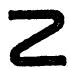
\includegraphics[keepaspectratio]{images/part002_45bf5402.jpg}}

注. 当集 H 满足命题 2 的条件时，它关于序 \(f \leqslant g\) 是一个格。但应指出，C 的子集 H 可以关于这个序是一个格，而 H 中两个函数 u、v 在 H 中的上确界（相应地，下确界）未必与它们在 C 中的上确界（相应地，下确界）相同。* R 的紧区间到 R 中的凸映射提供了一个例子。*

推论. 假设 H 满足：每当 \(u \in H\) 且 \(v \in H\) 时，有 sup \((u, v) \in H\) 与 inf \((u, v) \in H\) ；并且满足：对 X 的任意两个不同点 x、y 与任意两个实数 \(\alpha, \beta\) ，存在函数 \(g \in H\) 使得 \(g(x) = \alpha\) 且 \(g(y) = \beta\) 。则 X 上的每个连续实值函数都可用属于 H 的函数一致逼近。

定义 1. 若 X 是任意集合，X 到集合 Y 中的映射所成之集 H 称为分离 X 的子集 A 的元素（或称为 A 的元素的一个分离集），如果对 A 的任意两个不同元素 x、y，存在函数 \(f \in H\) 使得 \(f(x) \neq f(y)\) 。

例如，若 X 是完全正则空间（第 IX 章，§ 1，第 5 号），则 X 到 {[}0, 1{]} 中的全体连续映射所成之集分离 X 的点。

定理 2（斯通）. 设 X 是紧空间，H 是 C(X; R) 的向量子空间，使得 1) 常数函数属于 H；2) 若 \(u \in H\) ，则 \(|u| \in H\) ；3) H 分离 X 的点。则 X 上的每个连续实值函数都可用 H 中的函数一致逼近。

只需证明 H 满足命题 2 的推论的条件。由假设，若 \(u \in H\) 且 \(v \in H\) ，则有

\[
\sup (u, v) = \frac {1}{2} (u + v + | u - v |) \in H
\]

与

\[
\inf (u, v) = \frac {1}{2} (u + v - | u - v |) \in H.
\]

另一方面，设 \(x\) 与 \(y\) 是 \(X\) 的任意两个不同点，并设 \(\alpha, \beta\) 是任意两个实数。由假设，存在函数 \(h \in H\) 使得 \(h(x) \neq h(y)\) ：设 \(h(x) = \gamma\) ，\(h(y) = \delta\) 。由于常数属于 \(H\) ，函数

\[
g (z) = \alpha + (\beta - \alpha) \frac {h (z) - \gamma}{\delta - \gamma}
\]

属于 H 并且满足 \(g(x) = \alpha\) 与 \(g(y) = \beta\) 。

